\documentclass[11pt]{report}

%% Language and font encodings
\usepackage[english]{babel}
\usepackage[utf8x]{inputenc}
\usepackage[T1]{fontenc}
\usepackage[caption=false]{subfig}

%% Sets page size and margins
\usepackage[a4paper,top=3cm,bottom=2cm,left=3cm,right=3cm,marginparwidth=1.75cm]{geometry}
%% Useful packages
\usepackage{amsmath}
\usepackage{indentfirst}
\usepackage{graphicx}
\usepackage[colorinlistoftodos]{todonotes}
\usepackage[colorlinks=true, allcolors=blue]{hyperref}
\usepackage{setspace}
\usepackage{listings}
\usepackage{color}
\usepackage{subfig}
\usepackage{mathrsfs}
\usepackage{algorithm}
\usepackage[noend]{algpseudocode}
\usepackage{xfrac}
\usepackage{verbatim}
\usepackage[short]{optidef}
\algnewcommand\algorithmicinput{\textbf{Input:}}
\algnewcommand\algorithmicoutput{\textbf{Output:}}
\algnewcommand\Input{\item[\algorithmicinput]}%
\algnewcommand\Output{\item[\algorithmicoutput]}%
\newcommand{\sectionbreak}{\clearpage}

\date{}


\begin{document}
	\begin{titlepage}
		\begin{center}
    \Huge
    \textbf{Computational Mathematics for Learning and Data Analysis}

    \vspace*{1cm}

    \LARGE
        \textit{
        Implementation of a Neural Network optimized through Stochastic Gradient Descent and Conjugate Gradient
        Descent}

    \vfill

    
\includegraphics[scale=0.5]{img/cherubino_black.pdf}

    \vspace*{1cm}

    \Large
    Sabrina Briganti - 465214 - \href{mailto:brisabry5@gmail.com}{brisabry5@gmail.com}\\
    Gianmarco Ricciarelli - 555396 - \href{mailto:gianmarcoricciarelli@gmail.com}
    {gianmarcoricciarelli@gmail.com}

    \vspace*{1cm}

    \today
\end{center}

	\end{titlepage}

	\tableofcontents

	\chapter{The Artificial Neural Network} % (fold)
\label{cha:the_artificial_neural_network}
	In this first chapter, we provide some informations about the Artificial Neural Network, i.e. a fully
	connected Multilayer Perceptron, we implemented from scratch. We'll describe both the network's structure and
	the algorithm we used in order to make our network \textit{learn} from the data used during the testing and
	validation phases. Finally we'll present the loss function we have chosen for our network, and we'll provide
	and explanation on how it is differentiable. We'll use the notation proposed in \cite{Goodfellow-et-al-2016}.

	\section{The ANN's structure} % (fold)
	\label{sec:the_ann_s_structure}
		Since we have to write from scratch an \textit{Artificial Neural Network}, ANN for short, we have
		considered some alternatives before choosing the network's final structure. We agreed on a structure
		composed by:

		\begin{itemize}
			\item one \textit{input layer};
			\item two \textit{hidden layers};
			\item one \textit{output layer};
		\end{itemize}

		As convention, the number of units in the input layer is egual to the number
		of features of the dataset that is used for the learning, validation and testing phases. The two
		hidden layers contain, respectively, four and eight \textit{hidden neurons}, following the convention of
		putting an increasing series of powers of two as number of hidden units per layer. The number of neurons
		for the output layer depends on the kind of task the network is trying to fullfil. In the case of a
		\textit{classification task}, like the MONKS dataset \cite{Dua:2019}, we have decided to put one unit in
		the output layer, while in the case of a \textit{regression task}, like the CUP dataset, we have decided to
		put two units in the output layer. As we have seen studying the papers and books for gathering the
		necessary knowledge for the project, as \cite{Goodfellow-et-al-2016,haykin2009neural,mitchell1997machine},
		choosing to consider the network's structure as an \textit{hyperparameter}, that is, a variable, could
		lead to a series of difficult choices during the validation phase, so we have decided to fix the ANN
		structure to the one described for both the task we have to fullfil, changing only the number of units in
		the output layer from task to task. In figure \ref{fig:ann_structure} you can see our ANN's graph for
		the classification task.

		\begin{figure}
			\centering
			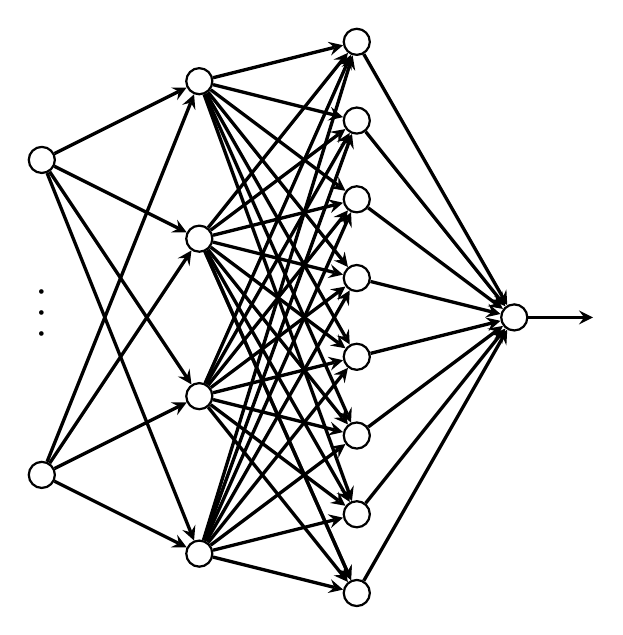
\begin{tikzpicture}
				\begin{scope}[every node/.style={circle,thick,draw}]
                    \node (A) at (-2,0) {};
                    \node (B) at (-2,-4) {};
                    \node (C) at (0,1) {};
                    \node (D) at (0, -1) {};
                    \node (E) at (0,-3) {};
                    \node (F) at (0,-5) {};
                    \node (G) at (2,1.5) {};
                    \node (H) at (2,0.5) {};
                    \node (I) at (2,-0.5) {};
                    \node (L) at (2,-1.5) {};
                    \node (M) at (2,-2.5) {};
                    \node (N) at (2,-3.5) {};
                    \node (O) at (2,-4.5) {};
                    \node (P) at (2,-5.5) {};
                    \node (Q) at (4,-2) {};
                \end{scope}

                \coordinate[right of=Q] (d1);

                \path (A) -- (B) node [black, font=\LARGE, midway, sloped] {$\dots$};

                \begin{scope}[>={stealth[black]},
                every edge/.style={draw=black,very thick}]
                    \path [->] (A) edge node {} (C);
                    \path [->] (A) edge node {} (D);
                    \path [->] (A) edge node {} (E);
                    \path [->] (A) edge node {} (F);
                    \path [->] (B) edge node {} (C);
                    \path [->] (B) edge node {} (D);
                    \path [->] (B) edge node {} (E);
                    \path [->] (B) edge node {} (F);

                    \path [->] (C) edge node {} (G);
                    \path [->] (C) edge node {} (H);
                    \path [->] (C) edge node {} (I);
                    \path [->] (C) edge node {} (L);
                    \path [->] (C) edge node {} (M);
                    \path [->] (C) edge node {} (N);
                    \path [->] (C) edge node {} (O);
                    \path [->] (D) edge node {} (P);
                    \path [->] (D) edge node {} (G);
                    \path [->] (D) edge node {} (H);
                    \path [->] (D) edge node {} (I);
                    \path [->] (D) edge node {} (L);
                    \path [->] (D) edge node {} (M);
                    \path [->] (D) edge node {} (N);
                    \path [->] (D) edge node {} (O);
                    \path [->] (D) edge node {} (P);
                    \path [->] (E) edge node {} (G);
                    \path [->] (E) edge node {} (H);
                    \path [->] (E) edge node {} (I);
                    \path [->] (E) edge node {} (L);
                    \path [->] (E) edge node {} (M);
                    \path [->] (E) edge node {} (N);
                    \path [->] (E) edge node {} (O);
                    \path [->] (E) edge node {} (P);
                    \path [->] (F) edge node {} (G);
                    \path [->] (F) edge node {} (H);
                    \path [->] (F) edge node {} (I);
                    \path [->] (F) edge node {} (L);
                    \path [->] (F) edge node {} (M);
                    \path [->] (F) edge node {} (N);
                    \path [->] (F) edge node {} (O);
                    \path [->] (F) edge node {} (P);

                    \path [->] (G) edge node {} (Q);
                    \path [->] (H) edge node {} (Q);
                    \path [->] (I) edge node {} (Q);
                    \path [->] (L) edge node {} (Q);
                    \path [->] (M) edge node {} (Q);
                    \path [->] (N) edge node {} (Q);
                    \path [->] (O) edge node {} (Q);
                    \path [->] (P) edge node {} (Q);

                    \path [->] (Q) edge node {} (d1);
                \end{scope}
			\end{tikzpicture}
			\caption{The ANN's structure for the classification task, the majority of the input nodes are
			omitted because they vary from dataset to dataset.}
			\label{fig:ann_structure}
		\end{figure}
	% section the_ann_s_structure (end)

	\section{Initializing the Network} % (fold)
	\label{sec:initializing_the_network}
		As we know from \cite{Goodfellow-et-al-2016,haykin2009neural,mitchell1997machine}, an ANN is composed by
		a set of weights $\mathbf{W}_{i}$, and a set of biases $\mathbf{b}_{i}$,
		$i \in \{ 1, \ \ldots \ , \ l \}$, with $l$ representing the ANN's number of layers. Although it is common
		practice to initialized the network's weights and biases to random, small, values, we have decided to
		follow the \textit{normalized initialization}, as described in
		\cite{Glorot10understandingthe,Goodfellow-et-al-2016}, which defines the initial values for the weights
		and the biases for each layer in the uniform distribution taken in the range

		\begin{equation*}
		    W \sim U \left [ -\frac{\sqrt{6}}{\sqrt{m + n}}, \ \frac{\sqrt{6}}{\sqrt{m + n}} \right ]
		\end{equation*}

		with $m$ and $n$, representing the number of inputs and outputs for each layer. This heuristic is
		designed to compromise between the goal of initializing all layers to have the same activation variance
		and the goal of initializing all layers to have the same gradient variance. The formula is derived using
		the assumption that the network consists only of a chain of matrix multiplications, with no
		nonlinearities. Other than this kind of initialization, we also make available the standard
		\textit{random initialization} for creating a network, described at the beginning of this section, which
		initialize the weights and the biases for each layer in the uniform distribution taken in the range

		\begin{equation*}
		    W \sim U \left [ - 0.7, \ 0.7 \right ].
		\end{equation*}
	% section initializing_the_network (end)

	\section{The back-propagation algorithm} % (fold)
	\label{sec:the_back-propagation_algorithm}
		The learning procedure for our ANN essentialy consist in two distinct phases:

		\begin{enumerate}
			\item compute the network's \textit{gradient}, that is, the derivative of the cost function
			$\nabla_{\theta} J(\theta)$, with $\theta$ representing the ANN's hyperparameters, with respect to
			every network's unit using the well known \textit{back-propagation algorithm}, described by
            algorithm \ref{alg:forward_propagation} and \ref{alg:backward_propagation};
			\item optimize the information gathered during the first phase using a distinct optimizer, chosen
			among the \textit{Stochastic Gradient Descent} and the \textit{Conjugate Gradient Method}, as
			described in chapter \ref{cha:optimizers};
		\end{enumerate}

		For computing the gradient we have chosen to use
		the well known \textit{backpropagation algorithm}, firstly introduced in \cite{10028086174} and described
		in \cite{Goodfellow-et-al-2016,haykin2009neural,mitchell1997machine}. This algorithm is
		also composed by two phases, a first phase, that is, the \textit{forward propagation}, in which the
		feature vector $\mathbf{x}$ given in input has to flow from the input layer through the hidden layers and,
		finally, the output layer, giving the approximation $\hat{\mathbf{y}}$ as output, and a second one, that
		is, the \textit{back-propagation}, which allows the information to flow backward through the network in
		order to compute the gradient by applying the Chain Rule of Calculus, that is, a technique for computing the
		derivative of a composition of functions.

		\begin{algorithm}[H]
			\caption{Forward propagation through a typical (deep) neural network and the computation of the cost
			function. Here $L(\hat{\mathbf{y}}, \mathbf{y})$ represents the loss function evaluated using both
			$\mathbf{y}$ and $\hat{\mathbf{y}}$ as inputs, more details about that will be provided in
			section \ref{sec:the_loss_function}. The function $f$ applied on line $5$ represents
			the layer's \textit{activation function}, while $\lambda \Omega(\theta)$ represents the
			network's regularization term, with $\theta$ representing the ANN's hyperparameters.}
			\label{alg:forward_propagation}
			\begin{algorithmic}[1]
				\Procedure{Forward propagation}{$l$, $\mathbf{W}_{i} \ i \in \{ 1, \ldots, l \}$,
				$\mathbf{b}_{i} \ i \in \{ 1, \ldots, l \}$, $\mathbf{x}$, $\mathbf{y}$}
					\State $\mathbf{h}_{0} = \mathbf{x}$
					\For{$k = 1, \ldots, l$}
						\State $\mathbf{a}_{k} = \mathbf{b}_{k} + \mathbf{W}_{k}\mathbf{h}_{k - 1}$
						\State $\mathbf{h}_{k} = f(\mathbf{a}_{k})$
					\EndFor
					\State $\hat{\mathbf{y}} = \mathbf{h}_{l}$
					\State $J = L(\hat{\mathbf{y}}, \mathbf{y}) + \lambda \Omega(\theta)$
				\EndProcedure
			\end{algorithmic}
		\end{algorithm}

		Since each one of the ANN's layers has its own
		\textit{activation function}, that is, a function that has to be applyied to the output of every layer's
		neuron, it is particularly usefull to think of the ANN like a composition of functions, and, for this
		reason, the Chain Rule of Calculus play a decisive role in the gradient's computation by back-propagation.
		It is import to note that with the term back-propagation we mean
		only the method for computing the gradient, not the whole learning algorithm. We now provide the
		pseudocode for the forward propagation and the back-propagation phases, as shown in algorithms
		\ref{alg:forward_propagation} and \ref{alg:backward_propagation}.

		\begin{algorithm}[H]
			\caption{Backward computation for the (deep) neural network of algorithm
			\ref{alg:forward_propagation}. Here, the $\odot$ symbol represents the element-wise
			(Hadamard) product, while $\nabla_{\hat{\mathbf{y}}}J =
			\nabla_{\hat{\mathbf{y}}}L(\hat{\mathbf{y}}, \mathbf{y})$ represents the gradient of the loss
			function computed with respect to the output $\hat{\mathbf{y}}$. $\nabla_{\mathbf{b}_{k}}J$,
			$\nabla_{\mathbf{W}_{k}}J$ and $\nabla_{\mathbf{h}_{k - 1}}J$ represents the gradient of the
			loss function computed with respect to, respectively, $\mathbf{b}_{k}$, $\mathbf{W}_{k}$ and
			$\mathbf{h}_{k - 1}$, and finally $\nabla_{\mathbf{b}_{k}} \Omega(\theta)$ and
			$\nabla_{\mathbf{W}_{k}} \Omega(\theta)$ represents the gradient of the ANN's hyperparameters computed
			with respect to, respectively, $\mathbf{b}_{k}$ and $\mathbf{W}_{k}$.}
			\label{alg:backward_propagation}
			\begin{algorithmic}[1]
				\Procedure{Backward propagation}{}
					\State $\mathbf{g} \leftarrow \nabla_{\hat{\mathbf{y}}}J = \nabla_{\hat{\mathbf{y}}}
					L(\hat{\mathbf{y}}, \mathbf{y})$
					\For{$k = l, l - 1, \ldots, 1$}
						\State $\mathbf{g} \leftarrow \nabla_{\mathbf{a}_{k}}J = \mathbf{g} \ \odot \
						f'(\mathbf{a}_{k})$
						\State $\nabla_{\mathbf{b}_{k}}J = \mathbf{g} \ + \ \lambda \nabla_{\mathbf{b}_{k}}
						\Omega(\theta)$
						\State $\nabla_{\mathbf{W}_{k}}J = \mathbf{g}\mathbf{h}_{k - 1}^{T} \ + \ \lambda
						\nabla_{\mathbf{W}_{k}} \Omega(\theta)$
						\State $\mathbf{g} = \nabla_{\mathbf{h}_{k - 1}}J = \mathbf{W}_{k}^{T}\mathbf{g}$
					\EndFor
				\EndProcedure
			\end{algorithmic}
		\end{algorithm}
	% section the_back-propagation_algorithm (end)

	\section{The activation functions} % (fold)
	\label{sec:the_activation_functions}
		As we have mentioned in section \ref{sec:the_back-propagation_algorithm}, each one of the ANN's layers
		has an \textit{activation function}, that is, a function that is applied to $\mathbf{a}_{k}$ in order to
		obtain $\mathbf{h}_k$, with $k \in \{1,\ldots,l\}$. We can say that an activation function of a node
		defines the output of that node, and maps $\mathbf{a}_{k}$ into the desired range. For being chosen as
		an activation function, a function has to possess a series of properties, such as

		\begin{itemize}
			\item \textit{nonlinearity}: when the activation function is non-linear, then a two-layer neural
			network can be proven to be a universal function approximator;
			\item \textit{range}: when the range of the activation function is finite, gradient-based training
			methods, such as the ones described in chapter \ref{cha:optimizers}, tend to be more stable, because
			pattern presentations significantly affect only limited weights;
			\item \textit{continuously differentiable}: since the functions have to be envolved in the Chain Rule
			of Calculus during the gradient's computation in the back-propagation algorithm;
		\end{itemize}

		There are many functions that can be used as activation functions for an ANN; we have chosen to utilize the
		well known \textit{logistic function}, i.e. the \textit{sigmoid function}, which is computed as

		\begin{align*}
		    &f(x) = \sigma(x) = \frac{1}{1 + e^{-x}} \\
		    &f'(x) = \sigma'(x) = f(x)(1 - f(x)),
		\end{align*}

		and is defined in the range $\left ( 0,\ 1 \right )$. As introduced in section
        \ref{sec:the_back-propagation_algorithm}, we can think the ANN as a \textit{composition} of activation
        functions, that is, representing it as

        \begin{equation*}
            \sigma_l \ \circ \ \sigma_{l - 1} \ \circ \ \cdots \ \circ \ \sigma_1
        \end{equation*}

        with $l$ representing the total number of layers in the network and $\sigma$ representing the logistic
        function.

	% section the_activation_functions (end)

	\section{The Loss function} % (fold)
	\label{sec:the_loss_function}
		It section \ref{sec:the_back-propagation_algorithm} we have referred to the \textit{Loss function} as to a
		function that takes as input the ANN's output vector $\hat{\mathbf{y}}$ and the \textit{ground truth}
		vector $\mathbf{y}$, that is, the vector containing the desired output for the network. But what
        essentially is a Loss function? As a matter of fact, the Loss function can be considered like
		one way of measuring the performance, or equivalently the error, of the model that utilizes it, an ANN in
		this case. There are various types of Loss functions, for our network we have decided to use a well
		known function: the \textit{Mean Squared Error}, MSE for short, for both the classification and the
        regression tasks. The MSE is obtained with the formula

		\begin{equation*}
		\label{mse}
		    \text{MSE} = \frac{1}{m}\sum_{i = 1}^{m}\left ( \hat{\mathbf{y}} - \mathbf{y} \right )^{2}_{i},
		\end{equation*}

		where $m$ represents the number of samples for which we computed the output $\hat{\mathbf{y}}$. We can
        represent this functions also as a composition of the square function and the Euclidean norm by writing
        the latter formula as

        \begin{equation*}
            \text{MSE} = \frac{1}{m}|| \hat{\mathbf{y}} - \mathbf{y} ||^2_2 .
        \end{equation*}

        Since this formula is used for computing the performances of our models, our primary goal is to minimize its
		output as much as possible by computing the gradient during the backward propagation step of the
		back-propagation algorithm, as described in section \ref{sec:the_back-propagation_algorithm}. Of course,
        in order to do so, it must be a \textit{differentiable} function. The gradient for the MSE with respect to
		$\hat{\mathbf{y}}$ is defined as:

		\begin{equation*}
		     \nabla_{\hat{\mathbf{y}}}\text{MSE}\left(\hat{\mathbf{y}},\ \mathbf{y}\right) =
		     \hat{\mathbf{y}} - \mathbf{y}.
		\end{equation*}

        \subsection{Properties of the Loss function} % (fold)
        \label{sub:properties_of_the_loss_function}
            Here we discuss the relevant properties of the Loss function we have chosen for our model.

            \begin{itemize}
                \item \textbf{Continuity}. As we introduced in this section, our Loss function is a function in
                two variables, $\hat{\mathbf{y}}$ and $\mathbf{y}$, respectively. A function $f$ in two variables
                is L-Lipschitz continuous if there exists a constant L such that

                \begin{equation*}
                    || f(\mathbf{x}_1, \mathbf{y}_1) - f(\mathbf{x}_2, \mathbf{y}_2) || \le L(|| \mathbf{x}_1 -
                    \mathbf{x}_2|| + || \mathbf{y}_1 - \mathbf{y}_2||) \quad \forall (\mathbf{x}_1, \mathbf{y_1}),
                    (\mathbf{x}_2, \mathbf{y_2}) \ \in \ \mathbf{dom} \ f.
                \end{equation*}

                Being the MSE a composition of the square function and the Euclidean norm, because of the squaring,
                the function is Lipschitz continuous only if we restrict its domain to a bounded set. Since, as
                described in section \ref{sec:the_activation_functions}, each network's layer uses the sigmoid
                function, which is a squashing function that bounds every layer's output in the range
                $\left ( 0,\ 1 \right )$, the MSE can be considered as a continous function.
                \item \textbf{Differentiability}. Again, being the sigmoid function the one used by the ANN,
                and since the sigmoid function is continuously differentiable with bounded Lipschitz continuous
                derivative, we can consider the MSE as a differentiable function, being the network a
                composition of continuously differentiable functions.
                \item \textbf{Convexity}. We recall that, for $h \ : \ \mathbb{R}^k \to \mathbb{R}$, $g_i \ : \
                \mathbb{R}^n \to \mathbb{R}$, the function:

                \begin{equation*}
                    f(\mathbf{x}) = h(g_1(\mathbf{x}), \ldots, g_k(\mathbf{x}))
                \end{equation*}

                is convex if $\mathbf{dom} \ h = \mathbb{R}^k$, $\mathbf{dom} \ g = \mathbb{R}^n$, $h$ is convex,
                $h$ is non-decreasing in each argument and $g_i$ are convex. For the aforesaid result, the squared
                Euclidean distance is convex, as any distance is non-negative and the square function is convex and
                increasing for non-negative values; however, when composed with another function it may not be
                convex. The functions that compose the network, that is, the sigmoid functions, are not convex
                functions, hence we can conclude that, for our network, the MSE is a not convex function.
            \end{itemize}

        % subsection properties_of_the_loss_function (end)

% chapter the_artificial_neural_network (end)

	\chapter{Optimizers} % (fold)
\label{cha:optimizers}
	\section{Stochastic Gradient Descent} % (fold)
	\label{sec:sgd}
		When choosing an optimizer, the \textit{Stochastic Gradient Descent}, SGD for short, is a quite common
		choice. It is not the best though, since, as proved by the last developments in the machine learning
		field, its convergence's rate is quite slow.
		Said that, it is also true that it allows to finds a very low value of the cost function quickly enough.

		The algorithm \ref{alg:sgd} shows the standard SGD version implemented, as described in
		\cite{Goodfellow-et-al-2016}, supporting both \textit{momentum} and \textit{regularization}.
		\cite{LIVIERIS2013491}

		SGD is an extension of the \textit{Gradient Descent Algorithm} (GD). It is an iterative first-order optimization technique, usefull to minimize the objective Loss function.

		The main goal is, indeed, to minimize the Loss function, in order to obtain a neural network with good generalization property:

		\begin{mini}
		  {\textbf{W}\in \mathbb{R}^n}{\textit{L}(\textbf{W}),}{\label{minimization}}{}
		\end{mini}

		where $\textit{L}$ is the Loss function and \textbf{W} are the synaptic weights of the network.

		The way to achieve this result, is to identify and compute a local minimum, moving along the direction of the steepest descent of the function, that is the negative gradient $-\nabla\textit{L}(\textbf{W})$.

		Of course, in order to find a local minimum, it is necessary to update the synaptic weights \textbf{W} at each iteration as $\textbf{W} = \textbf{W} +\Delta \textbf{W}$.

		The correction applied to the each one of the weights is defined as follows, taking a step in the opposite direction of the cost gradient:
		\begin{equation}
			\label{delta_rule}
			\Delta w_{ji} = -\eta \frac{\partial\textit{L}}{\partial w_{ji}},
		\end{equation}

		where $\eta$ is the learning rate. The latter one is a fundamental hyperparameter which has to been chosen wisely, since it represents how much is right to move along the descent direction: too much and the procedure will be vain, missing the minimum; too little and the converge will be slow.

		Unlike the GD algorithm, that could get a longer time to converges to the minimum because of the potentially big number of training examples, the SGD algorithm requires only the evaluation of one example for iteration (on-line mode).

		Here, however, we refer to SGD even when using the entire or just a subset of training dataset (batch or mini batch).

		The name stochastic derives from the fact that the samples are randomly selected, bringing to an approximation of the true gradient, estimated using a small set of samples. This is also the reason of the typical zig-zag pattern in the path towards the minimum of the Loss function, as visible in Fig.\ref{fig:gradient}.
		\begin{figure}
			\centering
		    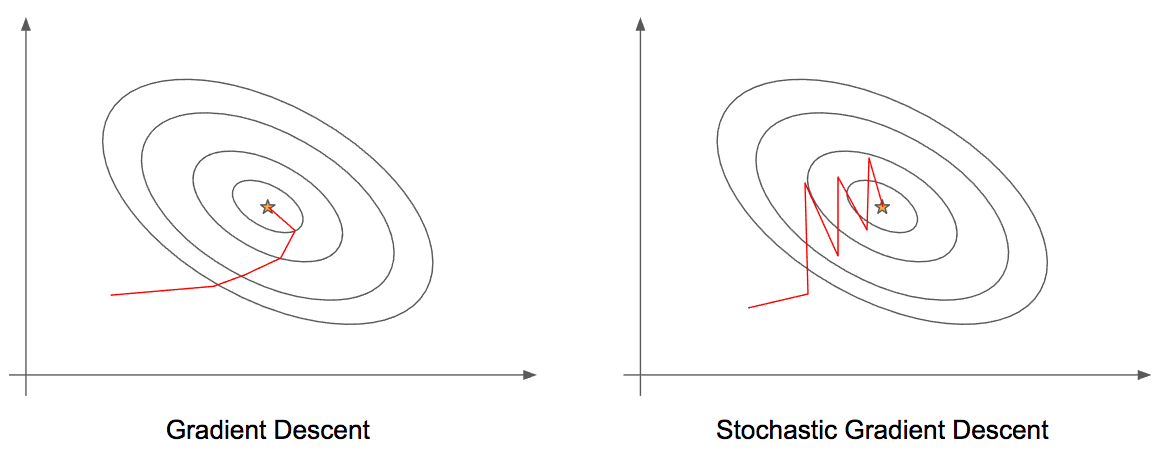
\includegraphics[width=.8\linewidth, scale=0.7]{img/figures/gradient.png}
			\caption{The different trajectories from GD and SGD.}
			\label{fig:gradient}
		\end{figure}
		%Due to its stochastic nature, c. However, it has been shown that SGD almost surely converges to the global cost minimum if the cost function is convex (or pseudo-convex)[1] [1] Bottou, Léon (1998). "Online Algorithms and Stochastic Approximations". Online Learning and Neural Networks. Cambridge University Press. ISBN 978-0-521-65263-6

		For what concernes the convergence of the stochastic gradient descent algorithm, it depends on the choice of $\eta$: it is necessary to gradually decrease the learning rate over the iterations for ensure convergence.
%deeplearning
		A sufficient condition to guarantee convergence of SGD is that the sequence of decreasing learning rates satisfy:

		\begin{equation}
			\label{delta}
			\sum_{t=1}^\infty \eta_t = \infty \text{  } \text{ and }\text{  } \sum_{t=1}^\infty \eta_t^2 < \infty
		\end{equation}

		%The cost function C(w) is three times differentiable with continuous derivatives.4 It is bounded from below, i.e. C(w) ≥ Cmin. We can assume, without loss of generality, that C(w) ≥ 0 - Online Learning and Stochastic Approximations, Leon Bottou
		Futhermore, if we assume that the Hessian matrix of the Loss function is strictly positive definite at the optimum, which means that the Loss function is strogly convex, the convergence rate is $O(\frac{1}{k})$, with \textit{k} as the number of iterations in the training. %strongly convex
		Otherwise, relaxing this assumption in presence of a convex problem, the convergence rate becomes $O(\frac{1}{\sqrt[]{k}})$\cite{Goodfellow-et-al-2016,Montavon:2012:NNT:2480981,Saad:1999:OLN:304710}.

		Unfortunatly, as we showed in \S\ref{sub:properties_of_the_loss_function}, our objective function is not convex, so we can't rely on what has been written before. Anyway, this issue seems to be overcomed: as proved in \cite{1606.04838}, the SGD is convergent even in presence of nonconvex functions.
		If the algorithm is run with a stepsize sequence satisfying Eq.\ref{delta} and the following assumptions hold:

		\begin{asu} - \label{as:conv}
  				If the level set $\mathcal{L} = \{w : \textit{L}(\textbf{W}) \leq L(\textbf{W}_1)\}$ is bounded,
  				in some neighborhood $\mathcal{N}$ of $\mathcal{L}$ the objective function \textit{L} is
  				continuously differentiable, and its gradient is Lipschitz continuous, there exist a constant $B >
  				0$ s.t. $\|\nabla\textit{L}(\textbf{W})-\nabla\textit{L}(\widetilde{\textbf{W}})\| \leq B\|
  				\textbf{W}-\widetilde{\textbf{W}}\| , \forall \textbf{W},\widetilde{\textbf{W}} \in \mathcal{N}$ ;
		\end{asu}

		\begin{asu} - \label{as:sgd_conv2}
				The Loss function \textit{L} and SGD satisfy:

				\begin{itemize}
					\item The sequence of weights ${\textbf{W}_k}$ is contained in an open set over which \textit{L} is bounded below by a scalar value $\textit{L}_{inf}$, that means the function is bounded below over the region explored by the algorithm;
					\item There exist scalars $\mu_G \geq \mu > 0 $ s.t., $\forall k \in \mathbb{N}$,
						\begin{equation}
							\nabla\textit{L}(\textbf{W}_k)^T\mathbb{E}_{\xi_k}[\textbf{g}(\textbf{W}_k,\xi_k)] \geq \mu \|\nabla\textit{L}(\textbf{W}_k)\|^2 \text{ and }
						\end{equation}
						\begin{equation}
							\|\mathbb{E}_{\xi_k}[\textbf{g}(\textbf{W}_k,\xi_k)]\|\leq \mu_G \|\nabla\textit{L}(\textbf{W}_k)\|,
						\end{equation}
					\item There exist scalars $M \geq 0 $ and $M_G \geq 0 $ s.t.:
						\begin{equation}
							\|\mathbb{V}_{\xi_k}[\textbf{g}(\textbf{W}_k,\xi_k)]\|\leq M + M_G\|\nabla\textit{L}(\textbf{W}_k)\|^2, \forall  k \in \mathbb{N},
						\end{equation}
				\end{itemize}

		\end{asu}

		then the following property is garanteed:

			\begin{equation*}
			     \lim_{k\to\infty}\mathbb{E}[\|\nabla\textit{L}(\textbf{W}_k)\|^2] = 0
			\end{equation*}

		that is the convergence of the algorithm.

		As we introduced in section \ref{sec:the_activation_functions}, each one of the units of our ANN uses
		the sigmoid function as activation function. This function bounds every layer's output in the range
		$(0, 1)$. In section \ref{sec:the_loss_function}, we have proved that our loss function is both
		Lipschitz continuous and differentiable. We can conclude that assumption \ref{as:conv} is respected.
		The first requirement of assumption \ref{as:sgd_conv2} is respected, being $L$ bounded in the
		interval $(0, 1)$, that is, having $L_{\mathit{inf}}$ eguals to $0$. The second requirement
		means that the vector \textbf{−g} (the extimate of the real gradient vector) is a direction of
		sufficient descent for \textit{L} with a norm comparable to the norm of the gradient. This property holds choosing $\mu_G = \mu = 1$ since, using SGD, $\textbf{g}(\textbf{W}_k, \xi_k)$ is an unbiased estimate of $\nabla L(\textbf{W}_k)$, while the
		third requirement restricts the variance of \textbf{g}, allowing it to assume non-zero values.
		At the time being, we are not able to further analyze the clauses of Assumption \ref{as:sgd_conv2}.

		A property of SGD is that the computation time per update does not grow with the number of training
		examples, allowing convergence even in presence of a large dataset.

		\begin{algorithm}[H]
			\caption{Stochastic Gradient Descent Algorithm. The learning rate $\eta$, the $\alpha$ term and the maximum number of iterations are given.}
			\label{alg:sgd}
			\begin{algorithmic}[1]
				\Procedure{Stochastic Gradient Descent}{}
					\State Initialize \textbf{W} and \textbf{v}
					\State $k \gets 0$
					\While {$k < max\_iterations$}
						\State Sample a minibatch of \textit{m} training examples \{\textit{$(x_0,y_0),(x_1,y_1),...,(x_m,y_m)$}\}
						\If {Nesterov Momentum}
							\State $\textbf{W} \gets \textbf{W} + \alpha \textbf{v}$
						\EndIf
						\State Compute gradient estimate: $\textbf{g} \gets \frac {1}{m} \nabla \sum_i\textit{L}(\textbf{W})$
						\State Compute velocity update: $\textbf{v} \gets \alpha \textbf{v} - \eta \textbf{g}$
						\State Apply update: $\textbf{W} \gets \textbf{W} + \textbf{v}$
					\EndWhile
				\EndProcedure
			\end{algorithmic}
		\end{algorithm}


		\subsection{Momentum}
		\label{sec:momentum}
			When computing the adjustment of the synaptic weights $\Delta\textbf{W}$ as in Eq. \ref{delta}, the choice of the learning rate $\eta$ influences the convergence of the SGD algorithm.
			The smaller is $\eta$, the smaller will be the changes in the matrix of weights and the rate of learning, but the smoother will be the trajectory.

			On the contrary, a bigger $\eta$ will bring to a faster convergence, but also to an oscillatory behaviour.

			A way to accelerate the SGD is the use of the \textit{Classical Momentum} (CM), a first order optimization technique which accelerate gradient descent, and so the learning rate of the final training.

			It consists in the adjustment of the new weigths through a velocity vector \textbf{v} that accumulates the gradient elements in the directions of reduction of the Loss function, and in a momentum coefficient $\alpha \in [0,1]$: the larger is  $\alpha$, the more the previous gradients affect the current direction.

			In this case, the classical momentum is given by:

			\begin{equation}
				\label{classical_momentum}
				\textbf{v}_k = \alpha\textbf{v}_{k-1} + \eta\nabla\textit{L}(\textbf{W}_k).
			\end{equation}

			The new synaptic weights are then updated as:
			\begin{equation}
				\label{update_momentum}
				\textbf{W}_k = \textbf{W}_{k-1}  + \textbf{v}_k.
			\end{equation}

			A variant of the CM algorithm, is the \textit{Nesterov's Accelerated Gradient} (NAG), which allows to avoid the oscillatory behaviour in the trajectory computed with CM, as visible in Fig.\ref{fig:momentum_graph}%fig2 on the importance}.

			The velocity vector \textbf{v} is computed as:

			\begin{equation}
				\label{nesterov_momentum}
				\textbf{v}_k = \alpha\textbf{v}_{k-1} + \eta\nabla\textit{L}(\textbf{W}_k + \alpha\textbf{v}_{k-1}).
			\end{equation}

			The update of the weights \textbf{W} follows the one described in Eq. \ref{update_momentum}.

			The variant respect Eq. \ref{classical_momentum}, shown in Fig.\ref{fig:momentum}, is given by the fact that the gradient $\nabla\textit{L}$ is evaluated after the current velocity is applied: NAG first update the $\textbf{W}_k$, making a jump in the direction of the previous accumulated gradient, and then evaluate the gradient in that point and makes a correction. This procedure allows it to change velocity vector $\textbf{v}_{k}$ in a faster way.

			We now discuss the convergence of a SGD using both classic momentum or Nesterov's accelerated
			gradient by providing some of the results illustrated in \cite{unified_convergence}, in particular
			the ones describing the case of the optimization of a non-convex function
			with Lipschitz continuous gradient, that is, our case.
			We denote by $\mathbb{E}[\cdot]$ the expected value taken with respect to the distribution of the
			random variable whose observed value represents the choice of a particular minibatch at step $k$ and by
			$\mathbf{g}_{k}$ the estimate of the true full-batch gradient $\nabla \mathcal{L}(\textbf{W}_{k})$ .

			Theorem \ref{theorem_1} ensures that SGD with or without momentum converges in expectation for non-convex functions, at the time being, we are not able to further analyze the Theorem's
			assumptions.

			\begin{theorem}[Convergence of Gradient Methods for Non-Convex Functions]
				Suppose $\mathcal{L}$ is a function with L-Lipschitz continuous gradient,
				$\mathbb{E} \left [ || \mathbf{g}_{i} - \nabla \mathcal{L}(\textbf{w}_{i}) ||^2 \right ] \le \delta^2$, and
				$|| \nabla \mathcal{L}(\textbf{w}_{i}) || \le G$ for any $\textbf{w}_{i} \in \textbf{W}$. Then, for any constant
				$C > 0$, running for k iteration the stochastic gradient method

				\begin{enumerate}
					\item with step size $\eta = \text{min} \left \{ 1\slash(2L),\ C\slash\sqrt{k + 1} \right \}$
					yields
					\begin{equation*}
					    \text{min}_{i = 0, \ldots, k} \mathbb{E} \left [ || \nabla \mathcal{L}(\textbf{w}_i) ||^2 \right ]
					    \le \frac{2(\mathcal{L}(\textbf{w}_{0})) - \mathcal{L}_{*}}{k + 1} \text{max} \left\{ 2B,\
					    \frac{\sqrt{k + 1}}{C} \right\} + \frac{CL\delta^2}{\sqrt{k + 1}} \ and
					\end{equation*}
					\item with step size $\eta = \text{min} \left \{ (1 - \alpha)\slash(2L),\
					C\slash\sqrt{k + 1} \right \}$ and a momentum $\alpha \in [0, 1)$ yelds
					\begin{align*}
						&\text{min}_{i = 0, \ldots, k} \mathbb{E} \left [ || \nabla \mathcal{L}(\textbf{w}_{i}) ||^2 \right ]
						\le \frac{2(\mathcal{L}(\textbf{w}_{0}) - \mathcal{L}_{*})(1 - \alpha)}{k + 1}
						\text{max} \left\{ \frac{2L}{1 - \alpha},\ \frac{\sqrt{k + 1}}{C} \right\} + \\
						&\frac{C}{\sqrt{k + 1}}\frac{L\alpha^2 + L\delta^2(1 - \alpha)^2}{(1 - \alpha)^3}
					\end{align*}
				\end{enumerate}
				\label{theorem_1}
			\end{theorem}

			It's worth to underline that, in case of batch mode and convex functions, Nesterov momentum brings the rate of convergence from $O(\frac{1}{k})$ (after k steps) to $O(\frac{1}{k^2})$\cite{10029946121}. % Nesterov, Y. (1983) A Method for Solving a Convex Programming Problem with Convergence Rate O(1/K2) . Soviet Mathematics Doklady, 27, 372-367.
			\begin{figure}
			\centering
				\begin{subfigure}[b]{0.4\textwidth}
					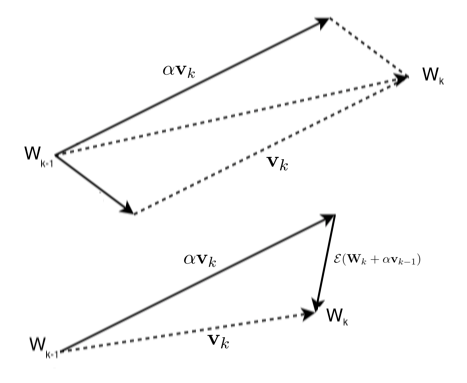
\includegraphics[width=\textwidth]{img/figures/momentum}
			  		\caption{The classical momentum on top and the Nesterov Accelerated gradient on bottom.}
				\label{fig:momentum}
				\end{subfigure}
				\qquad
				\begin{subfigure}[b]{0.4\textwidth}
					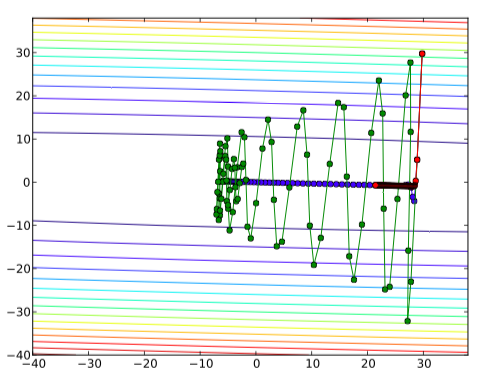
\includegraphics[width=\textwidth]{img/figures/momentum_graph}
				    \caption{The trajectory from CM (in green) and the one from NAG (in blue).}
				\label{fig:momentum_graph}
				\end{subfigure}
			\end{figure}


		\subsection{Regularization}
		\label{sec:regularization}

			In order to garantee a tradeoff between goodness and complexity of the model, the regularization is allowed in the network. This choice is important to ensure that the model doesn't grow too much in complexity.

			Regularization, in fact, adds a penalty as the model's complexity increases, forcing some weights to take values close to zero,  if they have little influence on the newtork performance and so resulting in poor generalization.

			It basically modifies the objective Loss functions as follows:

			\begin{mini}
				{\mathbf{W} \in \mathbb{R}^n} {\ \mathit{L}(\mathbf{W}) + \lambda\Omega(\mathbf{W})}{}{}
				\label{eq:reg}
			\end{mini}
			where $\Omega(\textbf{W})$ is a complexity penalty term based of the weights, and $\lambda$ is a parameter which tells how much importance must have the complexity penalty term.

			Two kinds of regularization are tipically used:

			\begin{itemize}
				\item \textit{L1}: also called Lasso Regression, which results in $\Omega(\textbf{W}) = \sum_{i=1}^{k} |w_i| = \|\textbf{W}\|_1$;
				\item \textit{L2}: also known as Ridge Regression, which results in $\Omega(\textbf{W}) = \sum_{i=1}^{k}w_i^2 = \|\textbf{W}\|_2^2$.
			\end{itemize}

			The addition of squared terms to the Loss function of Eq.\ref{mse} in the Ridge Regression, returns again a smooth continous and differentiable function. %Stochastic Gradient Descent and Regularization - Stanford CS Theory.Tim Roughgarden  Gregory Valiant

			However, the Lasso penalty, which pushes several elements of \textbf{W} to be exactly zero, making the result a sparse parameter vector, is not differentiable. So, since when applied to the Loss function, it returns a non-smooth function, it hasn't been tested on SGD\cite{journals/jmlr/Shalev-ShwartzT11}.

	\section{Nonlinear Conjugate Gradient}
	\label{sec:nonlinear_conjugate_gradient}

		An intresting optimization ables to lead to an improvement of the performances of the neural network, is the use of high-order information during the training phase: this brings to a more accurate choice of the search direction and of the step size, by using information from the second order approximation.

		In order to avoid the expensive computation of the inverse of the Hessian, we can use the \textit{Conjugate Gradient} methods, which are a class of iterative second-order optimization methods, derived from the steepest-descent algorithm, that ensure low memory requirements.

		In this way, the adjustment to the synaptic weights of the network is computed as:
		 \begin{equation}
		 	\label{weight}
		    \Delta\textbf{W} = \alpha\textbf{d},
		 \end{equation}
		where $\alpha$ is the learning rate and \textbf{d} is the new direction found.

		In our case, the nonlinear conjugate gradient methods are designed to solve the minimization problem defined in Eq.\ref{minimization}.

		As showed in the pseudocode \ref{alg:cgd}, the iterative formula generates a sequence of weights $\{W_k\}$, for every iteration of training \textit{k}, as:

		\begin{equation}
			\textbf{W}_{k+1} = \textbf{W}_{k} + \alpha_k\textbf{d}_k, \text{  }\text{  }\text{  } \textit{k} = 0,1,...,
		\end{equation}

		where $\alpha_k$ is a learning rate and $\textbf{d}_k$ is a descent direction. These are the new synaptic weights computed with the adjustment of Eq.\ref{weight}.

		% Because the error function E(~,) is nonquadratic, the algorithm will not necessarily con- verge in N steps. If the algorithm has not converged after N steps, the algorithm is restarted, i.e., initializing fik+J to the current steepest descent direction ~k+~  A Scaled Conjugate Gradient Algorithm for Fast Supervised Learning p4

		\begin{algorithm}[H]
			\caption{Nonlinear Conjugate Gradient Algorithm. The maximum number of iterations and the tolerance are given. $\sigma_1$ and $\sigma_2$ are two hyperparameters required in the LS procedure.}
			\label{alg:cgd}
			\begin{algorithmic}[1]
				\Procedure{Nonlinear Conjugate Gradient}{}
					\State Initialize $\textbf{W}_0$ and $\textit{L}_g$
					\State $k \gets 0$, $g_0 \gets 0$
					\While {$k < max\_iterations$}
						\State Evaluate the Loss function $\textit{L}_k$ and its gradient $\textbf{g}_k$
						\If {$\textit{L}_k < \textit{L}_g \text{ } \text{ or } \text{ } \|\textbf{g}_k\|> tolerance$}
							\State
							\Return Error goal reached
						\EndIf
						\State Compute the $\beta$ with one of the methods HS, MHS, FR, PR

						\State Compute the direction: $\textbf{d}_k \gets - \textbf{g}_k + \beta\textbf{d}_k$
						\State Compute the learning rate $\alpha_k$ with a Line Search satisfying the Strong Wolfe conditions, as discussed in \ref{sub:line_search}:
						\begin{equation*}
							\textit{L}(\textbf{W}_k+\alpha _k\textbf{d}_k)\leq \textit{L}(\textbf{W}_k)+\sigma_1\alpha\textbf{g}_k^T\textbf{d}_k
						\end{equation*}
						\begin{equation*}
							|\textbf{g}(\textbf{W}_k+\alpha_k\textbf{d}_k)^T\textbf{d}_k|\leq \textit{L}(\textbf{W}_k)+\sigma_2|\textbf{g}_k^T\textbf{d}_k|
						\end{equation*}

						\State Update the weights: $\textbf{W}_{k+1} \gets \textbf{W}_{k} + \alpha_k\textbf{d}_k$
						\State $k \gets k + 1$
					\EndWhile
				\EndProcedure
			\end{algorithmic}
		\end{algorithm}


		\subsection{Search Direction}
		\label{sub:search_direction}
			The direction $\textbf{d}_k$ holds the sequent property:
			\begin{equation}
			\textbf{d}_k^T\textbf{H}\textbf{d}_{tk-1} = 0,
			\end{equation}

		 	that means it is conjugate to the previous direction $\textbf{d}_{k-1}$. Furthermore, it doesn't need to know all the 	previous directions, but it only needs the last one, which is why it requires very little storage and computation.

			When dealing with quadratic functions, this method keeps the progress obtained so far in the minimization of the Loss function, by ensuring that the gradient along the previous direction does not increase.
			Anyway, it's worth to underline that this method can also be applyed with nonlinear functions: in this case, it should be necessary to restart the process, since there is no assumption that the conjugate directions previously found are still at the minimum of the function.

			Each new direction it's a linear combination of the steepest descent -\textbf{g} and the previous direction $\textbf{d}_{k-1}$, and it is defined as:
			\begin{equation}
			\label{dir}
			  \textbf{d}_k=\begin{cases}
			    -\textbf{g}_0, & \text{if $k=0$};\\
			    -\textbf{g}_k + \beta_k\textbf{d}_{k-1}, & \text{otherwise,}
			  \end{cases}
			\end{equation}

			where $\beta_k$ is a scalar, to be determined, that says how much of the previous direction should be added to the newest one. When applied to minimize a strictly convex quadratic function, it ensure that the directions $\textbf{d}_{k}$ and $\textbf{d}_{k-1}$ are conjugate with respective to the Hessian of the objective function, that is the property \ref{sub:search_direction} holds.

			Of course, the first search direction when $k = 0$ is defined as the steepest descent direction at the initial weight $\textbf{W}_0$ while, for $k > 1$, a minimization along each of the search direction is performed.

			Since it may be that the direction found is not a descent direction of the objective function, another modified search direction, proposed by Zang et al.\cite{L-2006}, has been tested in the project. It ensures sufficient descent $g_k^T = -\|g_k\|^2$, indipendent of the line search used or the convexity of the objective function, and is defined as follows:

			\begin{equation}
			\label{mod_dir}
				\textbf{d}_k^+=\begin{cases}
			    -\textbf{g}_0, & \text{if $k=0$};\\
			    -(1 + \beta_k\frac{\textbf{g}_k^T\textbf{d}_{k}}{\|\textbf{g}_k\|})\textbf{g}_k + \beta_k\textbf{d}_{k-1}^+, & \text{otherwise.}
			  \end{cases}
			\end{equation}



		\subsection{Beta}
		\label{sub:beta}
			What really makes the difference in the computation of the conjugate gradient algorithm, is the choice of the method used to compute the $\beta$ coefficient.

			In fact, there has been proposed various choices for computing it, each one giving different efficiency and properties.

			The formulas tested in our implementation are three: the Polak-Ribierère (PR), the Hestenes-Stiefel (HS) and a Modified Hestenes-Stiefel ($MHS^+$).

			One of the properties that must be garanteed, is the global convergence of the method. When the function to be minimized is convex and quadratic, indeed, the Conjugate Gradient algorithm ensures the convergence and the detection of the global minimum in at most N iterations, that is the number of dimensions. Often, expecially when N is very large, there are great chances that the algorithm terminates in less than N iterations.
			\cite{DIXON-1975}.
			However, since in our network we are dealing with a nonquadratic Loss function, as showed in \S\ref{sub:properties_of_the_loss_function}, the direction computed as in Eq. \ref{dir} could not be a descent direction. In order to avoid this issue, all the methods have been modified as follows, ensuring the global convergence \cite{doi:10.1137/0802003}:
			\begin{equation}
			\label{beta_max}
				 \beta^+ = max\{\beta, 0\}.
			\end{equation}

			This change provides a sort of restart of the algorithm, in case the $\beta$ found is negative. This is equivalent to forget the last search direction and start again the search from the steepest descent direction. The use of $\beta$ in Eq. \ref{beta_max} is similar to adopt the strategy of restarting the algorithm after N steps, initializing $d_k$ to the current steepest descent direction
			\cite{MOLLER1993525,Gilbert-1992}.

			\begin{equation}
			\label{betas}
				 \beta^{PR}_k = \frac{\textbf{g}_k^T(\textbf{g}_k-\textbf{g}_{k-1})}{\|\textbf{g}_{k-1}\|^2}, \text{ }
 				 %\beta^{FR}_k = \frac{\|\textbf{g}_{k}\|^2}{\|\textbf{g}_{k-1}\|^2}, \text{ }
 				 \beta^{HS}_k = \frac{\textbf{g}_k^T(\textbf{g}_k-\textbf{g}_{k-1})}{(\textbf{g}_k-\textbf{g}_{k-1}^T\textbf{d}_{k-1})}.
			\end{equation}

			%Powell [Griffiths-1984] was able to show that the Polak-Ribire method with exact line searches can cycle infinitely without approaching a solution point. The same result applies to the Hestenes-Stiefel method, since the two methods are identical when (gk,dk-1) 0, which holds when line searches are exact
			The HS and the PR methods in Eq. \ref{betas} have very similar performances and they are two of the most efficient conjugate gradient methods, but they are not globally convergent for nonlinear function\cite{Griffiths-1984}. That's why the modification of Eq. \ref{beta_max} has been adopted\cite{Powell-1986}, since it enforces the descent property of the algorithm.
			Both the methods are formulated in such a way that, when occurring small steps, the search direction found is close to the negative gradient direction, getting a final step of decent size\cite{Gilbert-1992}.
			Moreover, the HS method is considered superior to other methods when applied to nonquadratic functions.

			If we assume the Assumption \ref{as:conv} and we use a $\beta$ HS or PR, modified as in Eq.\ref{beta_max} and a Line Search as the one described in \S\ref{sub:line_search}, then it holds the convergence of the algorithm as follows\cite{Gilbert-1992}:

			\begin{equation}
			\label{conv_cg}
			  \lim_{k \to \infty} \|\textbf{g}_k\| = 0,
			\end{equation}
			a weaker result with respect to the one involved with strongly convex functions, $\lim_{k \to \infty} \textbf{g}_k = 0.$
			%SupposethatAssumptions2.1hold. Considerthemethod(1.2)- (1.3) with/3k max{/3R,0}, and with a line search satisfying the Wolfe conditions (2.4)-(2.5) and the sufficient descent condition (4.1). Then liminf Ilgkll O.


			%For what concernes the FR method (also described in Eq.\ref{betas}), it requires a constrain on the parameters of the inexact line search procedure of section \ref{sub:line_search}, used to identify the right step length $\alpha$. In particular, it requires that $\sigma_1 < \sigma_2 < 0.5$ in order to garantee that the Armijo Wolfe conditions are satisfied, and it seems to be less efficient and robust than the other methods \cite{Boyd:2004:CO:993483}, chapter 5.
			%Anyway, by imposing this condition, the FR method is globally convergent even when dealing with nonlinear functions.

			The last method tested is the $MHS^+$, a modified version of the Hestenes-Stiefel one \cite{LIVIERIS2013491}.
			It garantees sufficient descent with inexact line search and is based on a modified secant equation which approximates the second order information of the Loss function with high order accuracy. Moreover, it is globally convergent.

			It is defined as follows:

			\begin{equation}
			\label{mhs}
 				 \beta^{MHS}_k = \frac{\mathbf{g}_k^T \widetilde{\textbf{y}}_{k-1}^*}{\mathbf{d}_{k-1}^T\widetilde{\textbf{y}}_{k-1}^*}.
			\end{equation}

			In order to better understand the formula \ref{mhs}, it's important to describe all the components involved in its definiton.

			When dealing with quasi-Newton methods, an approximation $\textbf{B}_{k-1}$ of the Hessian of the Loss function $\nabla^2\textit{L}_{k-1}$ is update such that $\textbf{B}_k$ satisfies the secant condition:

			\begin{equation}
			\label{secant_1}
 				\textbf{B}_k (\textbf{W}_k - \textbf{W}_{k-1}) = \textbf{y}_{k-1},
 			\end{equation}

 			where $\textbf{y}_{k-1}$ is defined as $\textbf{g}_k - \textbf{g}_{k-1}$.
%new quasi newton method for unconstrain-wei

 			Wei et al. \cite{Zengxi-2006} derived a class of modified secant condition:

			\begin{equation}
			\label{secant_2}
 				\textbf{B}_{k-1} (\textbf{W}_k - \textbf{W}_{k-1}) = \widetilde{\textbf{y}}_{k-1},
 			\end{equation}


			\begin{equation}
			\label{secant_2}
 			 \widetilde{\textbf{y}}_{k-1} =  \textbf{y}_{k-1} + \frac{\theta_{k-1}}{(\textbf{W}_k - \textbf{W}_{k-1})^T\textbf{u}}\textbf{u},
 			\end{equation}

 			with \textbf{u} a vector satisying $(\textbf{W}_k - \textbf{W}_{k-1})^T\textbf{u} \neq 0$ and $\theta_{k-1}$ defined as:
 			\begin{equation}
			\label{theta}
 			 \theta_{k-1} = 2(\textit{L}_{k-1} - \textit{L}_{k}) + (\textbf{g}_k + \textbf{g}_{k-1})^T(\textbf{W}_k - \textbf{W}_{k-1}).
 			\end{equation}


 			Since for $\|(\textbf{W}_k - \textbf{W}_{k-1})\| > 1$ the standard secant Eq.\ref{secant_1} better approximates $\nabla^2\textit{L}_{k-1}(\textbf{W}_k - \textbf{W}_{k-1})$ than the modified version in Eq.\ref{secant_2}, Livieris and Pintelas\cite{LIVIERIS2013491} proposed a modification of the equation in this way:

 			\begin{equation}
			\label{secant_3}
 				\textbf{B}_{k-1} (\textbf{W}_k - \textbf{W}_{k-1}) = \widetilde{\textbf{y}}_{k-1}^*,
 			\end{equation}

 			\begin{equation}
			\label{y_3}
 				\widetilde{\textbf{y}}_{k-1}^* = \textbf{y}_{k-1} + \rho_{k-1} \frac{max\{\theta_{k-1},0\}}{(\textbf{W}_k - \textbf{W}_{k-1})^T\textbf{u}}\textbf{u},
 			\end{equation}

 			where $\rho_{k-1} \in \{0,1\}$ is a parameter that switch between the standard secant equation Eq.\ref{secant_1} and the modified one Eq.\ref{secant_3}, setting $\rho_{k-1}$ as:

			\begin{equation}
			\label{rho}
			  \rho_{k-1} =\begin{cases}
			    1 , & \text{if }\|(\textbf{W}_k - \textbf{W}_{k-1})\| \leq 1;\\
			    0 , & \text{otherwise.}
			  \end{cases}
			\end{equation}

			Since the following assumptions are satisfied by the Loss functions in Eq.\ref{mse}:

			\begin{asu} - \label{as:1}
  				The level set $\mathcal{L} = \{w \in \mathbb{R}^n | \textit{L}(\textbf{W}) \leq L(\textbf{W}_0)\}$ is bounded, there exist a constant $B > 0$ s.t. $\|\textbf{W}\| \leq B, \forall \textbf{W} \in \mathcal{L}$;
			\end{asu}

			\begin{asu} - \label{as:2}
				If in some neighborhood $\mathcal{N} \in \mathcal{L}$, \textit{L} is differentiable and its gradient \textbf{g} is Lipschitz continuous, then there exists a constant $ L > 0 $ such that
				\begin{equation}
				\label{ass2}
				  \|\textbf{g}(\textbf{W})-\textbf{g}(\widetilde{\textbf{W}})\| \leq L\|\textbf{W}-\widetilde{\textbf{W}}\|, \forall \textbf{ W},\widetilde{\textbf{W}} \in \mathcal{N},
				\end{equation}
			\end{asu}
			if the conjugate gradient algorithm is performed using $MSH^+$ and computing the search direction $\textbf{d}^+$ (as defined by Eq.\ref{mod_dir}), with a Line Search satisying the Armijo-Strong Wolfe conditions (described in \S \ref{sub:line_search}), the following theorem holds, as discussed in \cite{LIVIERIS2013491}:

			\begin{theorem}
				Suppose that \ref{as:1} and \ref{as:2} hold. If $\{\textbf{w}_k\}$ is obtained by Algorithm $MHS^+$ method, then we have
			\end{theorem}

			\begin{equation}
			\label{conv_mhs}
			  \lim_{k \to \infty} \|\textbf{g}_k\| = 0,
			\end{equation}

			that is the convergence of the algorithm.

			Assumption \ref{as:1} is satisfied, since, as we have said before, our loss function is bounded in the
			interval $(0, 1)$, and hence the level set is also bounded. Assumption \ref{as:2} is also satisfied,
			having described the properties for our loss function in section \ref{sec:the_loss_function}.

		\subsection{Line Search}
		\label{sub:line_search}
			Once computed the new direction \textbf{d} involved in the new weights \textbf{W}+$\alpha$\textbf{d}, a line search has to be implemented in order to find the right step size which minimize the Loss function.

			The step size $\alpha$ is nothing more than a scalar: the learning rate for the conjugate gradient algorithm, which tells how far is right to move along a given direction.

			So, fixed the values of the weights \textbf{W} and the descent direction \textbf{d}, the main goal is to find the right value for $\alpha$ that is able to minimize the Loss function:

			 \begin{mini}
			   {\alpha}{\textit{L}(\textbf{W} + \alpha\textbf{d}).}{}{}
			 \end{mini}

			Of course, we have to deal with a tradeoff: we want a good reduction, but we can't spend too much time computing the exact value for the optimum solution. So, the smarter way to get it is to use an inexact line search, that try some candidate step size and accepts the first one satisfying some conditions.

			This search is performed in two phases:
			\begin{itemize}
			\item a \textit{bracketing phase}, that finds an initial interval containing a minimizer;
			\item an \textit{interpolation phase} that, given the interval, finds the right step length in it.
			\end{itemize}

			We decided to use one of the most popular line search condition: the \textit{Armijo-Wolfe} condition.

			The search for the better $\alpha$ is led by two condition:
			\begin{itemize}
			\item the \textit{Armijo} one:
			\begin{equation}
			\textit{L}(\textbf{W}_k+\alpha _k\textbf{d}_k)\leq \textit{L}(\textbf{W}_k)+\sigma_1\alpha\nabla \textit{L}_k^T\textbf{d}_k
			\end{equation}

			which ensure that $\alpha$ gives a sufficient decrease of the objective function, being this reduction proportional to the step length $\alpha$ and the directional derivative $\nabla \textit{L}_k^Td_k$.

			The constant $\sigma_1$ has been set $\sigma_1=10^{-4}$, since it is suggested in literature to be quite small.

			\item the \textit{Strong Wolfe} condition:
			\begin{equation}
			|\nabla \textit{L}(\textbf{W}_k+\alpha _k\textbf{d}_k)^T\textbf{d}_k|\leq \textit{L}(\textbf{W}_k)+\sigma_2|\nabla \textit{L}_k^T\textbf{d}_k|
			\end{equation}
			which garantees to choose steps whose size is not too small.

			It is also known as curvature condition and ensures that, moving of a step $\alpha$ along the given direction, the slope of our function if greater than $\sigma_2$ times the original gradient (if the slope is only slightly negative, the function cannot decrease rapidly along that direction, so it's better to stop the search).

			In this case, the constant $\sigma_2$ is equal to 0.1, since a smaller value gives a more accurate line search.
			Futhermore, having choosen the strong condition, which doesn't allow the derivative to be too positive, we are sure that the $\alpha$ found lies close to a stationary point of the function.
			\end{itemize}

			\begin{algorithm}
			\caption{Line Search satisfying the strong Wolfe conditions. $\alpha_1 > 0$ and $\alpha_{max}$ are given.}\label{alg:linesearch}
			\begin{algorithmic}[1]
				\Procedure{line\_search}{}
				\State $\alpha_0 \gets \textit{0};$
				\State $i \gets \textit{1};$
				\While {$i \leq max\_iter$}
				 		\State  $ \text{Evaluate}\textit{L}(\alpha_i);$
						\If  { $[\textit{L}(\alpha_i) > \textit{L}(0) + \sigma_1\alpha_i\nabla\textit{L}_0^Td_0] \text{  or  } [\textit{L}(\alpha_i)\leq \textit{L}(\alpha_{i-1}) \text{  and  } i>1]  $ }
							\State $\alpha_* \gets \textbf{zoom}(\alpha_{i-1},\alpha_{i});$
							\Return $\alpha_*; $
						\EndIf
						\State   $\text{Evaluate } \nabla\textit{L}_{i} $
						\If  { $|\nabla\textit{L}_{i}| \leq -\sigma_2\nabla\textit{L}_0^Td_0 $}
							\State $\alpha_* \gets \alpha_i; $
							\Return $\alpha_*; $
						\EndIf
						\If  { $\nabla\textit{L}_{i} \geq 0$ }
							\State $\alpha_* \gets \textbf{zoom}(\alpha_{i},\alpha_{i-1}); $
							\Return $\alpha_*; $
						\EndIf
						\If  { $(|\textit{L}_{i} - \textit{L}_{i-1}| \leq threshold$ }
							\State $\alpha_* \gets\alpha_{i}$
							\Return $\alpha_*;$
						\EndIf
						\State $\text{Choose  } \alpha_{i+1}  \in (\alpha_i, \alpha_{max});$
						\State $i \gets i+1; $
				\EndWhile
			\EndProcedure
			\end{algorithmic}
			\end{algorithm}


			\begin{algorithm}
				\caption{Zoom}
				\label{alg:zoom}
				\begin{algorithmic}[1]
					\Procedure{Zoom}{}
						\While{True}
							\State  $ \alpha_j \gets \textit{quadratic\_interpolation}(\alpha_{lo}, \alpha_{hi}); $
							\State $ \text{Evaluate }\textit{L}(\alpha_j);$
							\If{$\left [ \textit{L}(\alpha_j) > \textit{L}(0) + \sigma_1 \alpha_j
							    \nabla  \textit{L}_0^T d_0 \right ]$ or $\left [ \textit{L}(\alpha_j) \leq
							    \textit{L}(\alpha_{lo}) \right ]$}
							    \State $\alpha_* \gets \alpha_j; $
								\State \Return $\alpha_*; $
							\Else
								\State $\text{Evaluate } \nabla \textit{L}_j^T d_j; $
								\If{$\left | \nabla \textit{L}_j^T d_j \right | \leq -\sigma_2 \nabla
								    \textit{L}_0^T d_0$}
								    \State $\alpha_* \gets \alpha_j; $
									\State \Return $\alpha_*; $
								\EndIf
								\If{$\nabla \textit{L}_j^T d_j (\alpha_{hi}-\alpha_{lo}) \geq 0 $}
									\State $\alpha_{hi} \gets \alpha_{lo}; $
								\EndIf
								\If{$(|\textit{L}_{j} - \textit{L}_{0}| \leq threshold$}
									\State $\alpha_* \gets\alpha_{j}$
									\State \Return $\alpha_*;$
								\EndIf
							\EndIf
						\State $\alpha_{lo} \gets \alpha_{j}; $
			{}			\EndWhile
					\EndProcedure
				\end{algorithmic}
			\end{algorithm}

			The algorithm satisfing the Strong Wolfe conditions is implemented through the functions described in the pseudocodes \ref{alg:linesearch}, \ref{alg:zoom} and is based on the the algorithms presented in \cite{Boyd:2004:CO:993483}, chapter 3.

			Since two consecutive values may be similar in finite-precision arithmetic, we set a threshold in both the \texttt{line\_search} and the quadratic interpolation functions, which garantees that the algorithm stops if two values of $\alpha$ are too close or if the maximum number of iterations has been reached.

			%The \texttt{line\_search} function try to find and return a good $\alpha$; if it fails, it returns an interval in which continue the searching, invoking the \texttt{zoom} function, which decreases the size of the interval, until it finds and returns a good step length.

			%\texttt{Zoom} invokes another function, \texttt{interpolate\_alpha}, which is nothing more than the implementation of a bisection interpolation in order to find a trial $\alpha$ inside the given interval.





			% \begin{algorithm}
			% \caption{Interpolate}\label{bisection}
			% \begin{algorithmic}[1]
			% \Procedure{interpolate\_alpha}{}
			% \State $i \gets \textit{1};$
			% \While {$i \leq max\_iter$}
			% 	\State $\alpha_{mid} \gets (\alpha_{hi}-\alpha_{lo})/2$
			% 	\State  $ \text{Evaluate }\textit{L}(\alpha_{mid});$
			%  	\If  { $[\textit{L}(\alpha_{mid}) == 0]  \text{  or  }  [(\alpha_{hi}-\alpha_{lo})/2 < threshold] $ }
			% 			\Return $\alpha_{mid}; $
			% 	\EndIf
			% 	\State   $\text{Evaluate } \textit{L}(\_{mid}alpha_{lo}); $
			% 	\If  { $sign(\textit{L}(\alpha_{mid})) == sign(\textit{L}(\alpha_{lo}))$ }
			% 		\State $\alpha_{lo} \gets \alpha_{mid}; $
			% 	\Else
			% 		\State $\alpha_{hi} \gets \alpha_{mid}; $
			% 	\EndIf
			% 	\State $i \gets i+1; $
			% \EndWhile
			% \EndProcedure
			% \end{algorithmic}
			% \end{algorithm}

	\chapter{Experiments} % (fold)
\label{cha:experiments}
    In this final chapter we present the results we obtained by applying our model to the datasets we have used
    to validate and test our ANN, namely, MONKS and CUP. Other than the results, we also present some details
    about the validation phase for each one of the datasets. We enrich the presentation by adding some graphs
    of the ANN's performances during the experimental phase.

    \section{MONKS} % (fold)
    \label{sec:monks}
        Before delving into the details of the results we obtained by applying our model to the dataset, we
        provide some informations about the \textit{preprocessing routines} and \textit{validation schema} we
        decided to use. Here are the steps we followed in order to reach the final states of our analysis.

        \begin{enumerate}
            \item Since the MONKS datasets’ feature are categorical, that is, every feature’s value represents
            a class, not a numerical value, we preprocessed the three datasets by writing a script
            for applying a \textit{1-of-k encoding}, hence obtaining 17 binary input features.
            \item As a supplementary preprocessing phase, we have applied a \textit{symmetrization} to the
            matrix containing the dataset’s values, in order to ease the training during the validation phase
            by having a matrix of values closer to the symmetric behavior of the sigmoid function, which was
            introduced in section \ref{sec:the_activation_functions}.
            \item Since we have chosen to follow \cite{Bergstra:2012:RSH:2188385.2188395} for the
            hyperparameters' search during the validation phase, we first performed some
            \textit{preliminary trials} in order to have a glimpse on the best intervals for searching our
            model's hyperparameters. During this trials we manually varied the model's hyperparameters, e.g.
            the learning rate, the momentum constant and so on for the SGD and the rho constant for the CGD,
            and observed the resulting \textit{learning curves}. For this part of the analysis we have used
            the $20\%$ of the training set as validation set, and the remaining part for training the network.
            \item We then deepen the search using the most interesting intervals discovered during the
            preliminary trials in the validation phase by using our implementation of the (random)
            \textit{grid search algorithm}, in which we also used our implementation of the
            \textit{k-fold cross validation algorithm} (which follows the standard approach of using a value
            of 3 for the k parameter).
        \end{enumerate}

        Our validation schema for the MONKS dataset essentially consists in using the random grid
        search
        algorithm to investigate some random sampled "points" in the hyperparameters' space, evaluating the
        performances for each one of this points and finally selecting the best combinations of parameters
        based
        on the diffent metrics like \textit{generalization error}, \textit{accuracy}, \textit{precision},
        \textit{recall} and \textit{f1-score}. Both in table \ref{tab:monks_sgd} and table
        \ref{tab:monks_cgd} we can find the results for the application of our model to the MONKS dataset,
        using as optimizer, respectively, the Stochastic Gradient Descent and the Conjugate Gradient Method,
        represented in a succinct fashion. Each row correspond to a specific dataset. The values for both the
        MSE and the Accuracy are represented by taking the mean over 10 executions on each dataset using
        the final configurations for the hyperparameters obtained during the validation phase.

        \subsection{Results for Stochastic Gradient Descent} % (fold)
        \label{sub:results_for_stochastic_gradient_descent}

            \begin{table}[H]
                \centering
                \begin{subtable}{\textwidth}
                    \resizebox{\textwidth}{!}{
                        \begin{tabular}{| c | c | c | c | c | c | c | c | c |}
                            \hline
                            Task & Topology & Batch size & Activation & $\eta$ & $\alpha$ & $\lambda$
                            & MSE (TR - TS) & Accuracy (TR - TS) (\%) \\
                            \hline
                            MONK 1 & 17 -> 4 -> 8 -> 1 & batch & sigmoid & 0.61 & 0.83 & 0.0 & 0.018 - 0.026 &
                            97 \% - 95 \% \\
                            \hline
                            MONK 2 & 17 -> 4 -> 8 -> 1 & batch & sigmoid & 0.64 & 0.78 & 0.0 & 0.010 - 0.015 &
                            98 \% - 97 \% \\
                            \hline
                            MONK 3 & 17 -> 4 -> 8 -> 1 & batch & sigmoid & 0.66 & 0.86 & 0.0072
                            & 0.015 - 0.017 & 97 \% - 97 \% \\
                            \hline
                        \end{tabular}
                    }
                \end{subtable}
                \caption{Results for the Stochastic Gradient Descent.}
                \label{tab:monks_sgd}
            \end{table}

           In order to compare the results in a similar configuration between the SGD and the CG, we have decided to adopt only the batch mode for training the ANN.
            Futhermore, for efficiency related reasons we have decided to use the \textit{Nesterov momentum}, as
            described in \cite{Goodfellow-et-al-2016,Sutskever:2013:IIM:3042817.3043064}, both in the
            validation and testing phases. The regularization constant $\lambda$ is used only in the third
            dataset, since Monk 3 is the only one among the three that has noisy samples.


        % subsection results_for_stochastic_gradient_descent (end)

        \subsection{Results for Conjugate Gradient Method} % (fold)
        \label{sub:results_for_conjugate_gradient_method}

        \begin{table}[H]
                \centering
                \begin{subtable}{\textwidth}
                    \resizebox{\textwidth}{!}{
                        \begin{tabular}{| c | c | c | c | c | c | c | c | c |}
                            \hline
                            Task & Topology & Activation & $\beta$ & $\sigma_{1}$ & $\sigma_{2}$ & $\rho$
                            & MSE (TR - TS) & Accuracy (TR - TS) (\%) \\
                            \hline
                            MONK 1 & 17 -> 4 -> 8 -> 1 & sigmoid & MHS & 0.0001 & 0.27 & 0.67
                            & $9.84e^{-5}$ - 0.0021 & 100 \% - 100 \% \\
                            \hline
                            MONK 2 & 17 -> 4 -> 8 -> 1 & sigmoid & MHS & 0.0001 & 0.12 & 0.73
                            & $9.62e^{-5}$ - 0.0026 & 100 \% - 99 \% \\
                            \hline
                            MONK 3 & 17 -> 4 -> 8 -> 1 & sigmoid & MHS & 0.0001 & 0.24 & 0.27
                            & 0.0038 - 0.010 & 99 \% - 98 \% \\
                            \hline
                            MONK 1 & 17 -> 4 -> 8 -> 1 & sigmoid & HS & 0.0001 & 0.28 & 0.0
                            & $9.94e^{-5}$ - 0.00059 & 100 \% - 100 \% \\
                            \hline
                            MONK 2 & 17 -> 4 -> 8 -> 1 & sigmoid & HS & 0.0001 & 0.35 & 0.0
                            & $9.85e^{-5}$ - 0.0019 & 100 \% - 100 \% \\
                            \hline
                            MONK 3 & 17 -> 4 -> 8 -> 1 & sigmoid & HS & 0.0001 & 0.14 & 0.0
                            & 0.0033 - 0.011 & 99 \% - 98 \% \\
                            \hline
                            MONK 1 & 17 -> 4 -> 8 -> 1 & sigmoid & PR & 0.0001 & 0.11 & 0.0
                            & 0.014 - 0.030 & 97 \% - 94 \% \\
                            \hline
                            MONK 2 & 17 -> 4 -> 8 -> 1 & sigmoid & PR & 0.0001 & 0.21 & 0.0
                            & 0.050 - 0.059 & 97 \% - 88 \% \\
                            \hline
                            MONK 3 & 17 -> 4 -> 8 -> 1 & sigmoid & PR & 0.0001 & 0.12 & 0.0
                            & 0.040 - 0.048 & 97 \% - 90 \% \\
                            \hline
                        \end{tabular}
                    }
                \end{subtable}
                \caption{Results for the Conjugate Gradient Method.}
                \label{tab:monks_cgd}
        \end{table}

        For what concernes the results for the Conjugate Gradient Method, for all the configurations tested,
        the direction has been set to the modified one, since it's the one who gave better results in the preliminary tests.

        It's immediate to see the higher performances achieved by the modified $MHS^+$ method and by the $HS^+$ one, reaching an accuracy of 100\% in both
        the training and test sets. On the contrary, the $PR^+$ method performes worse than the Stochastic
        Gradient Descent, behaving as in presence of overfitting. Like in the results obtained from SGD, the third dataset tested (Monk 3) gets a little worse performances because of the presence of noise in it.
        Anyway, it's interesting to underline that these models are able to reach higher accuracies with the
        ability to "auto-tune" themeselves, that is without the necessity to modify at hand hyperparameters as the learning rate or the the momentum term.

        Another nice behaviour with respect to the one showed in SGD, is evident from the learning curves in Appendix \ref{cha:monks_learning_curves}: the Conjugate Gradient Methods reach the highest accuracy in the very first epochs, while the Stochastic Gradient Descent needs much more epochs of training to converge towards an optimum value.

        % subsection results_for_conjugate_gradient_method (end)
    % section monks (end)

% chapter experiments (end)

\end{document}